\leadauthor{Sanderson}

\title{Taxonium: a web-based tool for exploring large phylogenetic trees}
\shorttitle{Taxonium}

\author[1]{Theo Sanderson \orcidlink{0000-0003-4177-2851}}
\affil[1]{The Francis Crick Institute, UK}

\date{}

\maketitle

\begin{abstract}
The COVID-19 pandemic has resulted in a step change in the scale of sequencing data, with more genomes of SARS-CoV-2 having been sequenced than any other organism on earth. Previous web-based tools for phylogenetic exploration were not able to directly scale to this size of tree. We have developed Taxonium, a new tool that uses WebGL to allow the exploration of trees with tens of millions of nodes. Taxonium allows visualisation of mutation-annotated trees, where the genotypes at each internal node are indicated, and also links each node to associated metadata. An optional server-side backend permits rapid loading for widely used datasets, while a client-only mode allows the exploration of niche or sensitive data. Taxonium is an open-source tool which can be applied to any large tree. We provide an application for exploring a public tree of more than five million SARS-CoV-2 sequences at \href{http://cov2tree.org}{cov2tree.org}, the broader Taxonium tool at \href{http://taxonium.org}{taxonium.org}, and source code at \href{https://github.com/theosanderson/taxonium}{github.com/theosanderson/taxonium}.


\end{abstract}

\begin{keywords}
tree | visualisation | phylogenetics
\end{keywords}

\begin{corrauthor}
theo.sanderson\at crick.ac.uk
\end{corrauthor}

\section*{Introduction}\label{s:introduction}

Genomic researchers responded to the emergence of SARS-CoV-2 with rapid collaboration at unprecedented scale. Open protocols were quickly generated for amplicon sequencing \citep{Tyson2020}, and allowed researchers across the globe to produce ever-growing genomic datasets stored both in the INSDC databases \citep{insdc}, and in GISAID \citep{shu2017gisaid}, with the latter recently surpassing 11 million sequences. Importantly, new tools were also developed to understand the functional diversity of these samples, by assigning them into lineages proposed by the community \citep{rambaut2020dynamic, o2021assignment}, and allowing interactive exploration of trends in these data over time \citep{hodcroft_2021, chen2022cov, outbreakinfo}.

The vast scale of these datasets has posed challenges for the array of tools that researchers had previously relied upon to manipulate, analyse, and visualise genomic data. In particular, the construction of phylogenetic trees, and the visualisation of these trees, has been a bottleneck in the analysis of SARS-CoV-2 genomic data. There are two broad responses possible to this issue. One is to downsample the sequences analysed in order to create a smaller dataset with which existing tools are able to work efficiently. This has been an important approach, and has allowed NextStrain \citep{nextstrain} to provide one of the most widely-used and important tools for exploring SARS-CoV-2 genetic diversity. Briefly, the NextStrain pipeline downsamples sequences in a rational way, and then uses iqtree \citep{iqtree} to assemble them into a tree, assigns chronology and ancestral states to this tree using TreeTime \citep{treetime}, and displays the results in a user-friendly interactive interface using Auspice \citep{nextstrain}. All three of these post-downsampling stages are bottlenecks which prevent the use of full datasets, and so NextStrain analyses are typically limited to \textasciitilde4,000 nodes -- sampled in a structured way to ensure they either provide an overview of the pandemic or hone in on particular sequences of interest.

\begin{figure}

\begin{center}
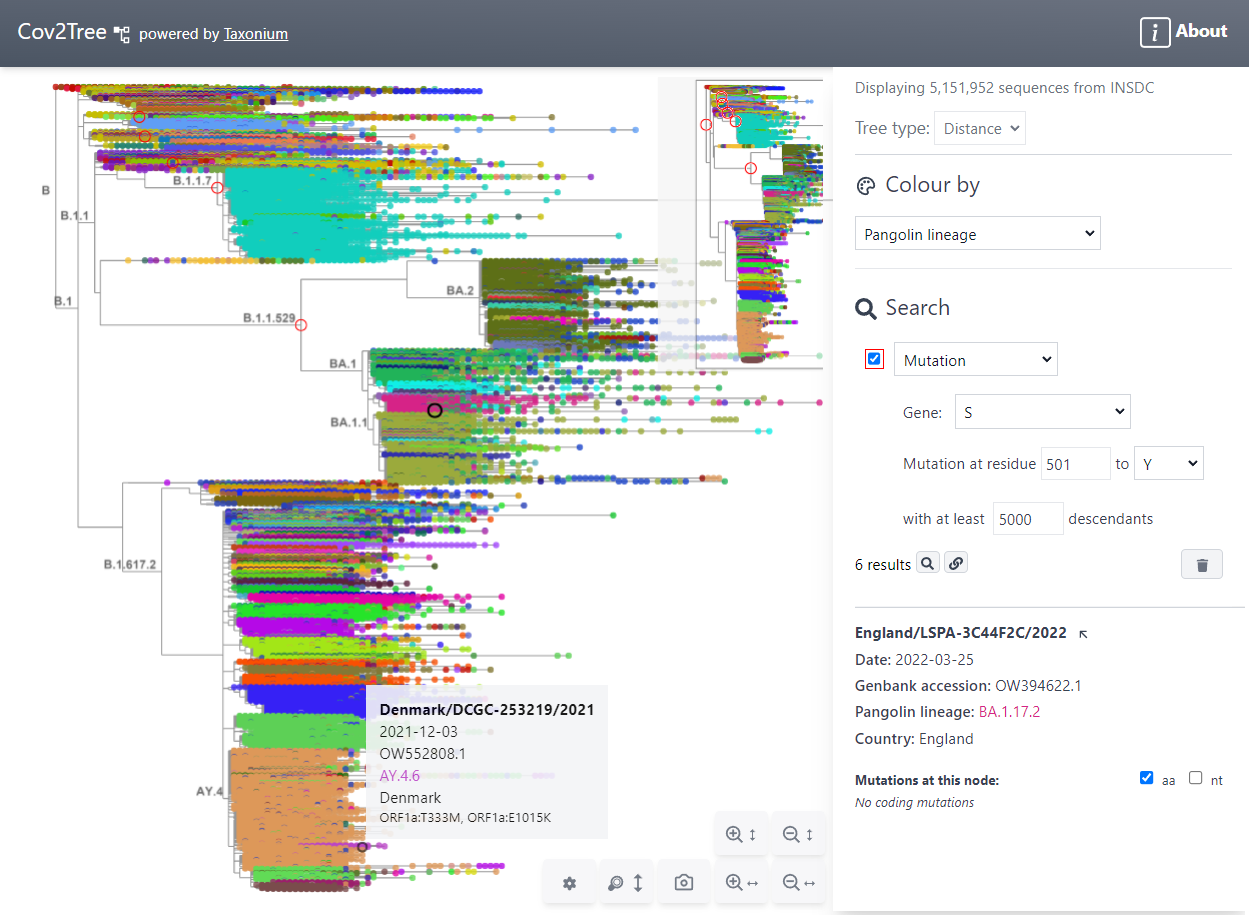
\includegraphics[width=\linewidth]{Figures/cov2tree.png}
\end{center}
\caption{The Taxonium web client displaying a 5,151,952 sequence tree of SARS-CoV-2 sequences. The left hand panel shows the zoomable tree with a minimap for orientation, and the right hand panel provides options for searching for nodes and for changing the colour scheme. Hovering over a node shows information in a tooltip, while clicking on a node displays further information in the right-hand panel. A search has been carried out for mutations at S:501 to Y, filtered to such nodes with 5,000 descendants, which are circled in red. Genomes are coloured by their PANGO lineage.}
\label{fig:taxonium_client}
\end{figure}

The new scale of data available provides an impetus to develop new tools that are able to work with these large datasets without downsampling. Recently the development of UShER \citep{usher} has permitted larger trees to be built than ever previously. UShER takes a starting tree, built with iqtree or a similar approach, and incrementally adds sequences by maximum parsimony. For densely sampled sequencing efforts, as in the SARS-CoV-2 pandemic, such an approach still yields tree topologies of very high quality \citep{Thornlow2021.12.02.471004}. To turn this distance tree into a time tree, by estimating a time associated with each node in the tree, we recently developed Chronumental \citep{chronumental} which uses stochastic gradient descent to efficiently construct chronologies from very large trees, which was not possible with previous approaches. A final necessary component is a tool for exploring these large trees, ideally in a browser.

Here we describe Taxonium, a web-based tool for for examining large trees. Taxonium scales to trees with millions of nodes, and allows for rapid panning and zooming using WebGL. In addition to reading Newick format trees, Taxonium can also display UShER mutation-annotated trees which capture genotype information in mutations at internal nodes. It permits searching for nodes by metadata or genotype, and a range of colouring options. Taxonium is available in a server-backed mode, which in a matter of seconds loads to allow exploration of all publicly available SARS-CoV-2 sequences, and also a fully client-side mode suitable for exploring custom datasets, including those with sensitive data.


\section*{Methods}\label{s:results}

\subsection*{The Taxonium Web Client}

The Taxonium web client is a React application for exploring trees. One major bottleneck of previous approaches was the use of web technologies involving SVG or Canvas to visualize the tree, which have performance limitations. We instead use WebGL, as implemented via DeckGL \citep{deckgl}, for efficient visualisation of the tree. Even so, rendering every node in the tree would still be too slow, and would involve hundreds of nodes overplotted on each pixel when a tree was zoomed out. We address this by rendering a sparsified version of the tree, with the sparsification dependent on the zoom level such that only nodes that would be hidden by other nodes are excluded. This approach allows for fast and responsive tree exploration.

The input to Taxonium is a tree (e.g. in Newick format) and, optionally, metadata. Metadata is associated with each node of the tree, and the tree can be coloured by any chosen metadata item. Colours are by default selected using an algorithm that hashes the metadata's string value into a unique colour, ensuring consistency over time without the need for comprehensive look-up tables. In addition, the tree can be searched based on the metadata, with identified nodes circled. Complex hierarchical boolean combination queries using AND, OR, or NOT  are supported.

\begin{figure}
\begin{center}
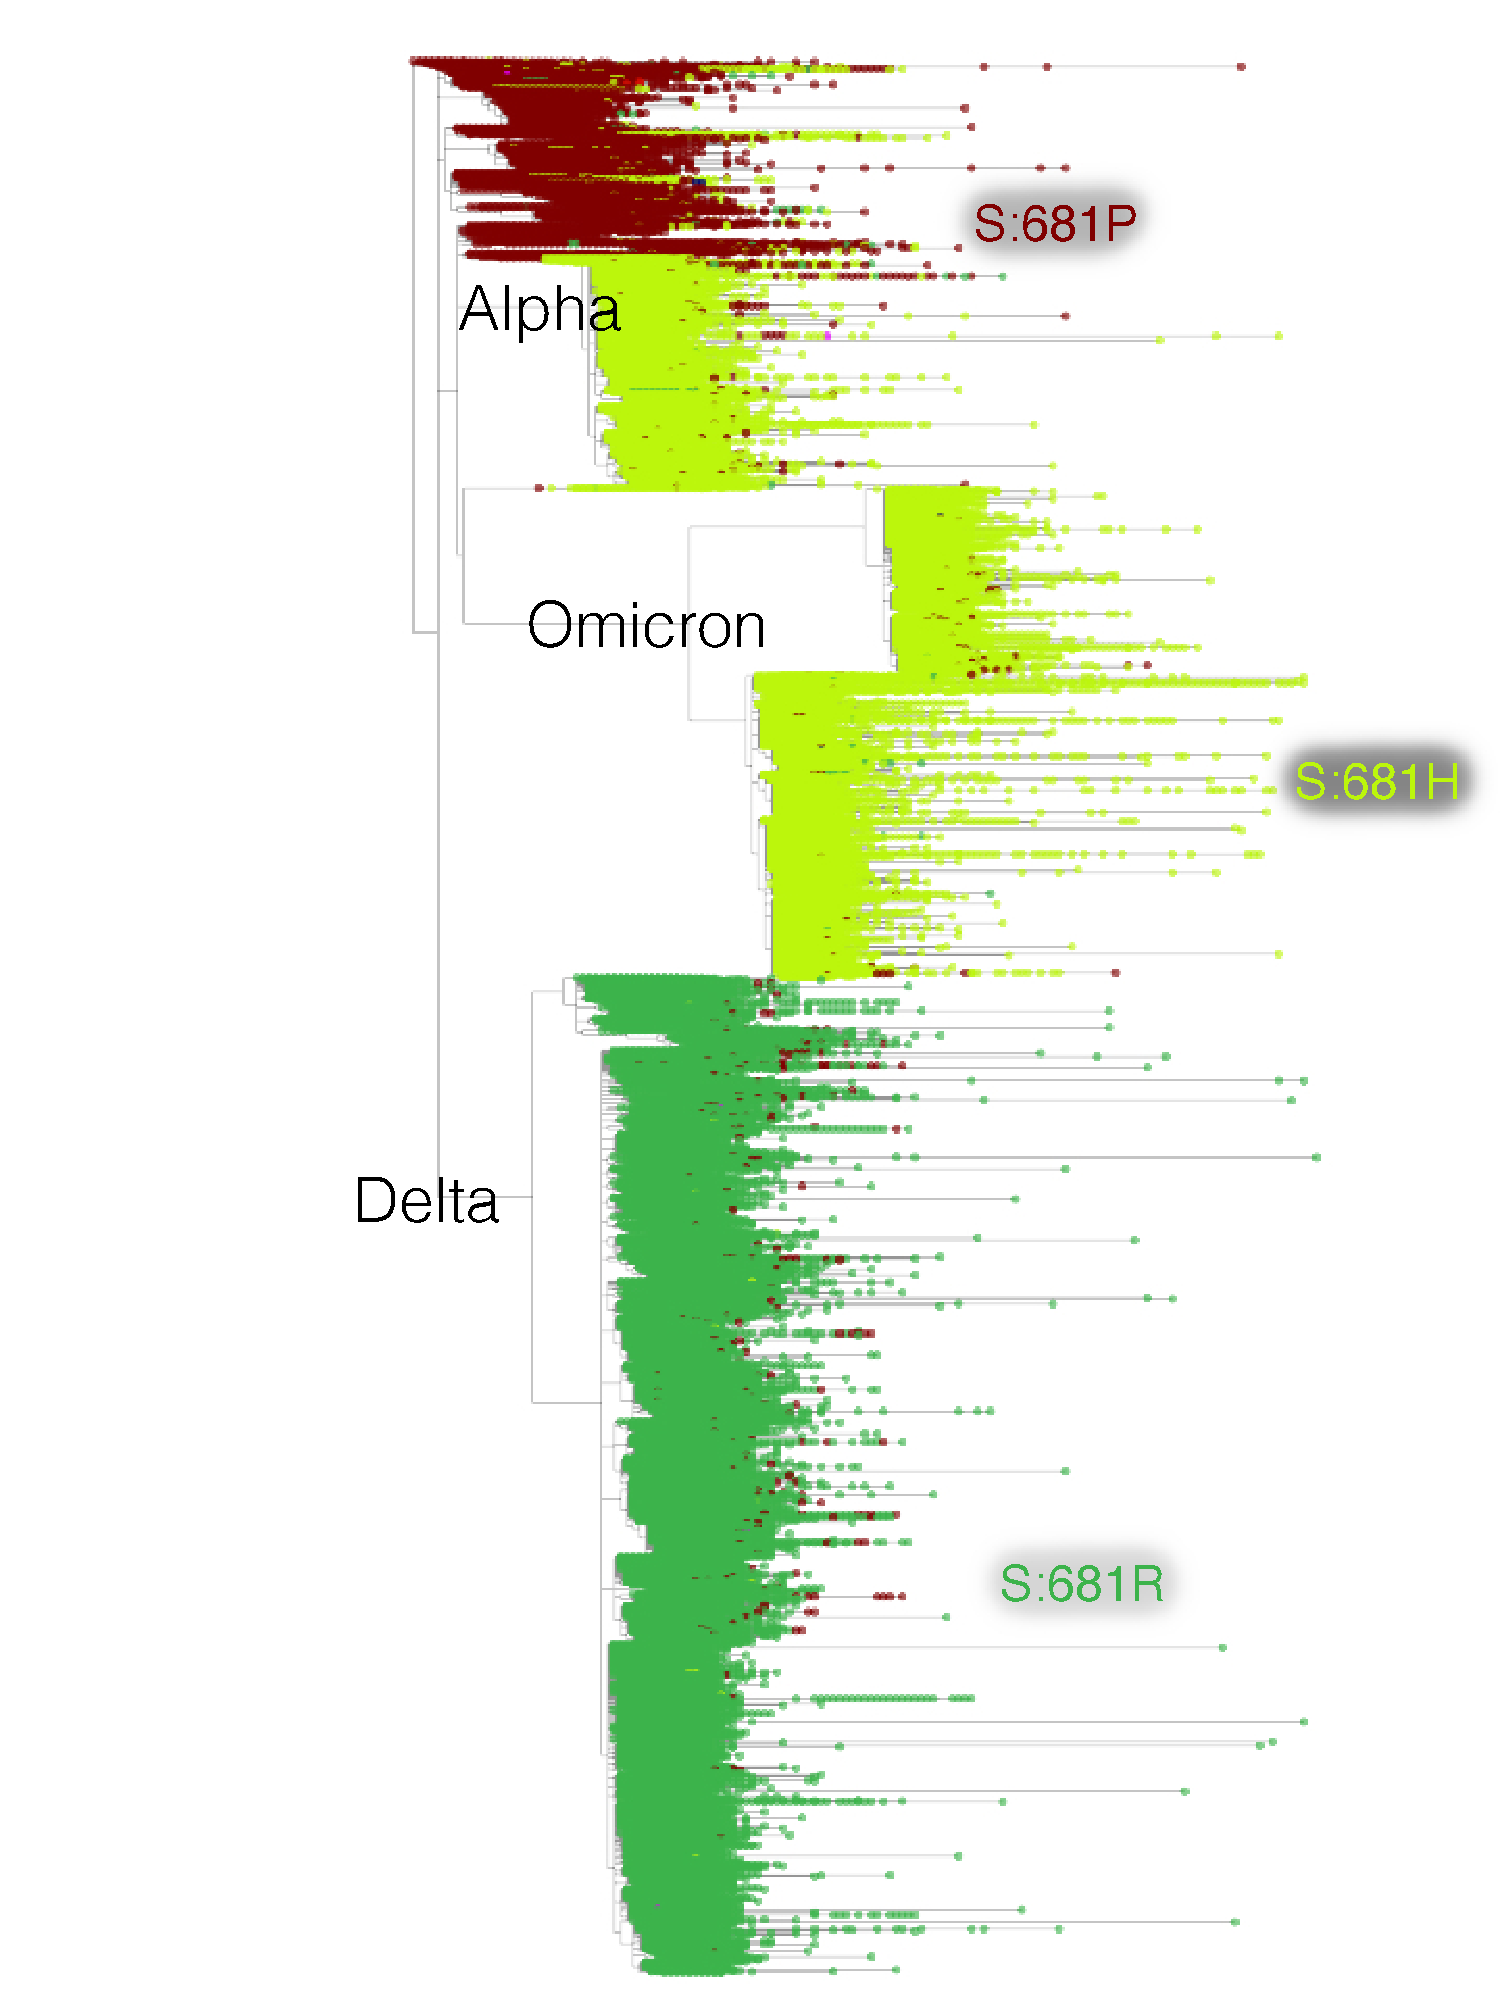
\includegraphics[width=0.9\linewidth]{Figures/681.pdf}
\end{center}
\caption{Overlaying genotype data at position Spike 681 on 4,616,067 SARS-CoV-2 genomes with Taxonium. Taxonium's `Colour by genotype' feature was used to generate this screenshot. Labels were added afterwards.}
\label{fig:681}
\end{figure}

The user interface of the Taxonium web client is shown in \cref{fig:taxonium_client}. The tree, at the left hand side of the screen, can be panned, and can be zoomed in the vertical and horizontal axes independently. The latter is a crucial feature for large trees, which are invariably much larger in their y-axis. A toggleable minimap is provided for orientation. The right hand panel allows users to search for nodes of interest, to select how the tree is coloured, and to select between a chronological and a distance tree. It also displays information about the selected node; similar information is available upon hovering over a node of interest.



In addition to accepting traditional trees, Taxonium also supports mutation annotated trees (MATs, \citet{matutils}), of the type generated by UShER, where internal nodes are annotated with mutations inferred to have occurred at that point in the phylogeny. Since an MAT essentially captures the full sequence of each sample in the tree, its use as an input permits the user to colour the tree by genotype at any desired site (\cref{fig:681}), or alternatively to search for particular mutations in internal modes (\cref{fig:452}), and to filter by how many leaf nodes these mutations gave rise to.



\begin{figure}
\begin{center}
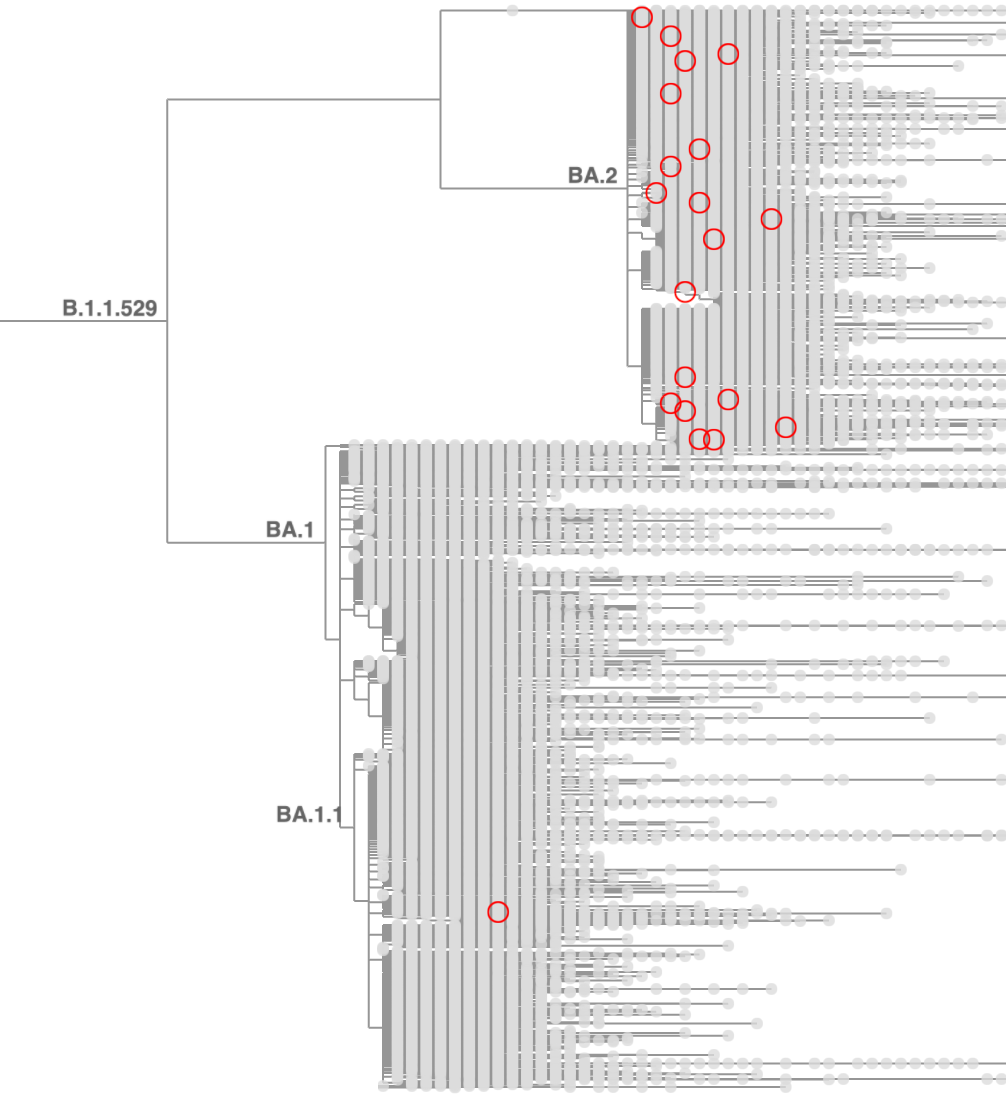
\includegraphics[width=\linewidth]{Figures/452_2.png}
\end{center}
\caption{Looking for recurrent mutations in SARS-CoV-2 with Taxonium. Here we have zoomed in on Omicron (B.1.1.529), with 1,422,024 sequences until late May 2022, and are circling nodes featuring a mutation at S:452 to either M or Q which have more than 10 descendants. These appear to be much more common on the BA.2 genetic background.}
\label{fig:452}
\end{figure}

Taxonium can allow visualisation of trees entirely in the client, which is especially important for trees which may contain sensitive patient-level data. Trees are loaded either from a Newick file and TSV metadata file, or from a custom preprocessed Taxonium JSONL format combining the two. The Taxonium JSONL format contains a pre-computed layout for the tree, reducing the amount of computation required for its display, but Newick files can also be laid out in the client, which is achieved using an approach heavily based on JStree \citep{jstree}. More expensive computational operations, such as the sparsification of the tree for display, are performed in a web worker in order to maintain a responsive interface.

\subsection*{The Taxonium Backend}

The client-side only version of Taxonium is highly responsive, and permits loading trees with millions of nodes on typical consumer computers. However, the process of deserialising tree data from disk into Javascript objects in memory is a bottleneck, requiring one minute and 20 seconds for a tree of 5.4 million sequences. Large trees also demand increasing amounts of RAM and download bandwidth which might rule out the use of lower spec devices. To allow near instantaneous access to trees with millions of nodes on almost any internet-connected device, we built a server-backed mode for Taxonium, in which a server reads trees from disk in advance and then serves required parts of them to each client on demand. The server-backed mode is more efficient, as it does not require all data to be sent to the client, and the computationally expensive operations can be performed on a more powerful machine. Using this mode, a 5.4 million sequence tree can initially load in seconds. We continue to offer the client-side mode, which has the advantage that it can be used with custom data, and especially for data that may be sensitive and not suitable for uploading.



The Taxonium backend is implemented in NodeJS using Express. It runs from the same codebase that runs in the web worker in the browser. We made substantial efforts to make this backend code as efficient as possible. Nodes are stored sorted by their y coordinates, meaning that two binary searches can be used to identify the slice of nodes that lie within a supplied window.

\subsection*{Taxoniumtools}

We provide a simple Python application, \texttt{taxoniumtools}, which allows straightforward generation of a Taxonium JSONL file from an UShER MAT. The Taxonium JSONL format combines tree topology, node metadata, and mutations, in a row-wise format. The tree's structure is encoded only in the \texttt{parent\_id} property of each node.

Taxoniumtools uses TreeSwift \citep{moshiri2020treeswift} for rapid loading of the Newick string located within the UShER MAT file. Optionally it can run Chronumental \citep{chronumental} as part of the building process and integrate the resulting time tree into the final JSONL file.

Full documentation for Taxonium and Taxoniumtools is available at \href{http://docs.taxonium.org}{docs.taxonium.org}.

\section*{Implementations}

We have implemented Taxonium in a several applications, which provide examples of some of the ways it can be useful.

\subsection*{Cov2Tree}

We used Taxonium to build the Cov2Tree web application (\href{http://cov2tree.org}{cov2tree.org}), which allows users to explore the global diversity of SARS-CoV-2 (Figure 2). 

Cov2Tree uses the UShER tree built by \cite{McBroome2021}, which currently contains 5.4 million sequences. We provide a time tree inferred by Chronumental, and also provide a daily-updated file containing the date placements inferred by Chronumental\footnote{\url{https://cov2tree.nyc3.cdn.digitaloceanspaces.com/chron_dates.tsv.gz}} which can allow the identification of sequences with metadata errors \citep{chronumental}.

We run a backend server that supports the Cov2Tree application, meaning that the user needs only to download the data for the region of the tree on which they have zoomed in. This helps to enable analysis in lower bandwidth settings. Users can colour the tree by PANGO lineage, by sample country, or by genotype, and use searches to conduct complex queries.

In the case of the SARS-CoV-2 dataset, the server backend requires around 5 GB of RAM per server instance.

\subsection*{Other projects}

We decided to use Taxonium to create a tool that allows exploration of the NCBI Taxonomy database \citep{federhen2012ncbi}. The resulting visualisation, which can be found at \href{http://taxonomy.taxonium.org}{taxonomy.taxonium.org}, allows interactive viewing of the taxonomic relationships between 2.2 million species, as well as searches.


We have also collaborated with the Serratus project \citep{edgar2022petabase} to allow visualisation of trees of virus sequences identified in a search of petabases of sequence from the Sequence Read Archive. Each viral order and family at \href{http://serratus.io/trees}{serratus.io/trees} now provides an option to open a custom Taxonium tree.

With the arrival of the 2022 monkeypox outbreak in Europe, we launched \href{http://mpx.taxonium.org}{mpx.taxonium.org} to allow exploration of an open genomic dataset from LAPIS \citep{lapis}.



\begin{figure}
\begin{center}
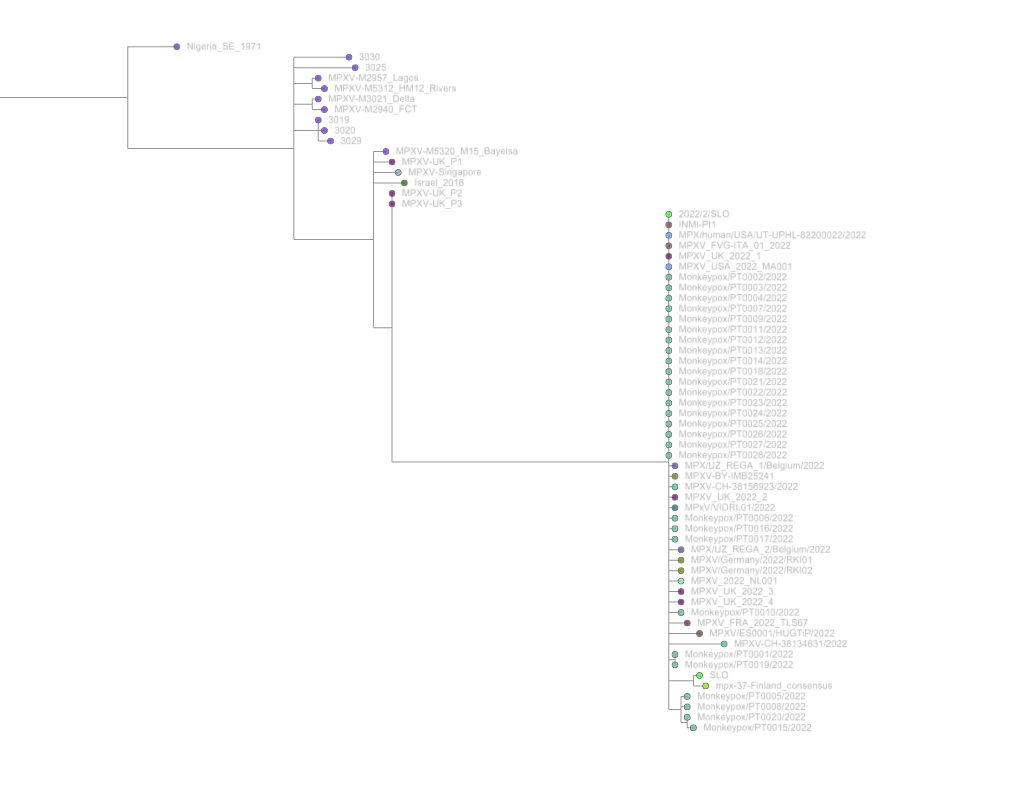
\includegraphics[width=\linewidth]{Figures/taxonium (4).png}
\end{center}
\caption{
A screenshot of the mpxTree application showing monkeypox phylogeny. 
}
\label{fig:cov2tree}
\end{figure}

\section*{Comparison to other tools}

\subsection*{Scale}

We argue that Taxonium is currently the tool that best scales to the largest trees. To examine this we here compare a number of tools for their ability to load a very large tree. We stress that many of these tools were likely not specifically designed to be able to load trees of this size, unlike Taxonium.

We used the example of a Newick tree derived from a recent UShER public tree \citep{McBroome2021} featuring 5,326,538 sequences \footnote{\url{https://hgwdev.gi.ucsc.edu/~angie/UShER_SARS-CoV-2/2022/05/17/public-2022-05-17.all.nwk.gz}}. On a Macbook Pro (2018 version, 2.3 GHz quad-core i5), Taxonium loaded this tree from the Newick file in 31 seconds. We were able to open this file with Dendroscope -- for which we increased its allotted RAM to 5 GB. The tree loaded in 1 minute and 23 seconds, however it rendered initially as a single black rectangle which only began to resolve upon zooming in, making it difficult to extract insights about the tree. Dendroscope used all available RAM whereas Taxonium used 1.7 GB. In general, Taxonium felt substantially more responsive.

We attempted to load the same file on Microreact.org \citep{argimon2016microreact} (which now uses Phylocanvas.GL), but the screen locked up and had not loaded within a reasonable time. A Phylocanvas.GL demo \footnote{\url{https://www.phylocanvas.gl/examples/very-large-tree.html}} does show that the library \citep{abudahab2021phylocanvas} is able to load a SARS-CoV-2 tree with >1M leaves, panning relatively slowly on our hardware.

Archaeopteryx \citep{archaeopteryx} took >5 minutes to load this tree with stack size set to 5 GB, and then was essentially unresponsive. Empress 1.20 \citep{CantrellFedarko2021empress} did not load this tree in the browser in any reasonable length of time. We were unable to upload this file to iTOL \citep{itol} or the ETE Tree Explorer \citep{ete}.

\subsection*{Features}

It must be noted that all these tools have different feature sets. Many of the tools above allow for features absent from Taxonium, such as re-rooting, displaying trees radially, collapsing subtrees, and more. Support for these features to an extent trades-off against scale. Conversely, Taxonium is unique among these tools in supporting mutation-annotated trees, and perhaps in its ability to toggle to a time tree -- features shared with, and inspired by, Auspice \citep{nextstrain}.

An array of other tools for tree visualisation exist, with diverse feature sets. We have aimed to test here those most likely to scale to the largest trees available. As an aside, we believe that vertical zoom is an all-but-essential feature for any tree viewer to be useful in exploring the detail of large phylogenies, but absent from a surprising number of tools.

\section*{Discussion}\label{s:discussion}

The increased scale of recent genomic datasets has prevented existing tools from being used to explore entire phylogenies in the case of SARS-CoV-2. While unprecedented, these SARS-CoV-2 datasets likely provide a preview of future data volumes for many other organisms given the decreasing costs of sequencing and increasing infrastructure for genomic surveillance.

Taxonium allows exploration of these large phylogenies, and is also one of few tools to allow the visualisation of a mutation-annotated tree capturing all known sequence diversity in an organism. It is open-source and highly configurable for use with any tree. We have used Taxonium to build the Cov2Tree website, which has been widely used to explore the global diversity of SARS-CoV-2.

Some tools for phylogenetic trees are designed primarily for generating static figures suited for publications. These may offer features Taxonium lacks, such as the ability to visualise phylogenies in a circular layout, and the ability to output vector graphics. In contrast, Taxonium is intended primarily for exploring a tree dynamically -- in the case of very large trees, this often the only way to extract useful information.

One challenge in this new era of vast datasets is the variable quality of sequences, and therefore resultant phylogenies. Artifacts in sequences (e.g. \citet{pmid35130474,sanderson2021variation,sanderson2021systematic}) are often systematic, and in such cases can create entire clades brought together by shared errors. Existing efforts to tackle these issues have been important, for example pooling knowledge of known sites of common spurious mutations \citep{de2020masking}. The development of new pipelines and assemblers that minimize artifacts will be important in the future, and the development of tree-building algorithms that are able to consider the possibility of variation due to artifacts, or pre-tree masking steps that mask different sites in each sequence, may be valuable. Widespread deposition of raw reads would allow systematic assembly by pipelines designed to minimise systematic errors. In Taxonium we provide a search option that highlights ``revertant'' mutations in which a branch apparently mutates back towards the reference genome. In large SARS-CoV-2 phylogenies, many of these mutations appear to in fact represent sequencing artifacts, or reversion from them, and so this approach may help identify areas of a tree that may have technical issues. 

Taxonium is an ongoing open source project to create and maintain a tree viewer able to scale to the latest phylogenies. We welcome contributions from the community and hope that the features described here will be useful to those working on epidemiological surveillance and outbreak response.


\small
\subsection*{Acknowledgements}

Phylogenetic analysis of viral genomes is only possible thanks to a community of researchers and clinicians who take viral samples, generate genomes, and submit to sequence databases such as the INSDC databases and GISAID, and I am very grateful to all contributors. I am indebted to Richard Goater for development advice and to Angie Hinrichs for maintenance of the underlying tree that powers Cov2Tree. This preprint uses a \href{https://github.com/roylelab/manuscript-templates}{LaTeX template} from the Royle Lab, which in turn was forked from a template by Ricardo Henriques.

This work was supported by the Wellcome Trust (210918/Z/18/Z) and the Francis Crick Institute which receives its core funding from Cancer Research UK (FC011104, FC011233), the UK Medical Research Council (FC011104, FC011233), and the Wellcome Trust (FC011104, FC011233).



\section*{Bibliography}
\bibliographystyle{bxv_abbrvnat}


\bibliography{refs.bib}